\documentclass[12pt,a4paper]{article}
\usepackage{amsmath,bm} %mathematische Normen
\usepackage[english]{babel} %neue deutsche Rechtschreibung und Formelsatz
\usepackage{amsfonts} %Zus�tzliche Formeln/Symbole/Sonderzeichen...
\usepackage{amssymb} %Formelsatz
\usepackage{graphicx} %Einbinden von Graphiken
\usepackage{float} %Flussumgebungen
\usepackage{cite}
\usepackage[font=footnotesize]{caption}
\usepackage{enumerate}
%\usepackage[utf8]{inputenc} %linux
\usepackage[ansinew]{inputenc} %windows
\usepackage[left=3cm,right=2.7cm,top=2.5cm,bottom=2.7cm,includeheadfoot]{geometry}

\date {\today}
\author{Veit L�schow}
\title{Heterogeneous core-mantle boundary heat flux in thermo-chemical core convection}

\begin{document}
\maketitle
\newpage
\tableofcontents
\newpage

\section*{Abstract}

Thermal coupling between convection in Earth's mantle and core was proposed to explain asymmetric features of the geomagnetic field during the history of the Earth. The coupling is caused by laterally varying heat transport from the core to the mantle, induced by lateral temperature gradients in the lower-most mantle. Clues for the temperature gradients were found by seismic tomography.\\
This numerical study aims to explore the influence of these non-uniform boundary conditions, as compared to uniform heat flux and isothermal boundary conditions on thermo-chemical core convection and some distinct dynamo properties. \\ 
In our model the heat flux pattern is modeled by a single spherical harmonic of degree and order 2. This setting conserves equatorial symmetry, but imposes azimuthal heat flux gradients. \\
Today, convection in the Earth's core is assumed to be driven predominantly by a combination of thermal and compositional buoyancy sources located at the inner-core boundary. Thermal and compositional diffusivities differ by orders of magnitude. The resulting differences in the dynamical behavior of the two components demand an approach with distinct transport equations and boundary conditions for temperature and chemical concentration. Simulations for five different ratios of thermal and chemical driving are made. \\
We observe that fixed flux conditions promote larger flow scales and an increase of mean kinetic energy densities. The imposed flux pattern locks the outer core flow to the mantle and therefore breaks its azimuthal symmetry, even for relatively low thermal forcing ratios of 20 \%. Despite of the symmetry breaking, stable and dipolar dynamos can be maintained due to the partly chemical forcing with its uniform boundary conditions. Additionally, the chemical component partly adopts to the geometry of the heat flux pattern because advective transport of concentration is more effective in regions of increased heat flux.

\section{Introduction}

\section{Things to write}

\begin{itemize}
 \item Model description 
 \item Motivation: Double diffusive, heat flux pattern
 \item Heat flux model: consequences for linear profile / convective profile
 \item Formation of vortex columns
 \item Influence of chemical forcing on dipolarity (Tr�mper)
 \item state of research
 \item Numerical solution scheme
 
\end{itemize}

 
\section{Modeling core convection and dynamo action}

Rotating convection and dynamo action in Earth's core is a topic that has been explored by many authors. There exist various ideas of how to formulate a set of equations that depicts all relevant physical processes and that is still as simple and therefore numerically economical as possible. Computation time is the limiting factor when it comes to the question how realistic models of the inner core can be made. The gap between the relevant physical parameters expected for the Earth and the parameters that are in range of numerical modeling is still big. It cannot be expected that this gap will be closed only with the help of increasing computational resources within the next years. Alternatives to waiting for larger computers that are able to cope with earth-like parameters have to be found. Asymptotic models are one possibility already revealing promising results.\\
A question that is closely related to the numerical costs and therefore to the accessible parameter range is the choice of the geometry. Most models are either Cartesian with periodic boundary conditions or spherical shell models. The latter are of course more realistic for the Earth but numerically more costly and therefore even less earth-like when looking at the reachable parameters. In this work, a spherical model is used in order to be as earth-like as possible in a geometrical way. As a trade-off, parameter regimes in which Cartesian models could advance, are unreachable here. \\
We model the electrically conducting liquid outer core. It is enclosed by the inner-core boundary (ICB) at the bottom and the core-mantle boundary (CMB) at the top. Convection is driven by destabilizing thermal and compositional gradients across the sphere. For the compositional component, fixed chemical concentrations at the ICB and the CMB are imposed (Derichlet boundary condition). The thermal forcing is maintained by introducing a fixed in - and out flux of heat (Neumann boundary condition). The heat flux at the CMB can be made laterally heterogeneous, i.e., there are regions of higher and lower than average heat flux. The inner core and mantle are assumed to be insulating and therefore have no influence on the evolution of magnetic fields. \\ 
In the following all relevant equations are introduced. There exist numerous detailed derivations so that this description will be held relatively short.\\
\subsection{Frame of reference}
The liquid outer core (LOC) is modeled with the help of a spherical shell with an inner radius R$_i$ and an outer radius R$_o$. It is bounded by the ICB at the bottom the CMB at the top. The shell thickness is chosen according to what is expected for today's state of the Earth and defined over the ratio between R$_i$ and r$_o$: $ a = $ R$_i$ / R$_i$ = 0.35.\\
The LOC is constantly rotating about the z-axis of a Cartesian system. The angular velocity $\Omega$ is invariant in time. The effect of the rotation on the frame of reference will be discussed when it comes to the equation of motion. In the course of this study,it is quite nearby to chose spherical coordinates. 
\begin{figure}[]
 \begin{minipage}{0.45\textwidth}
  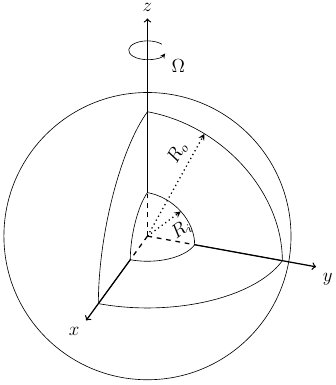
\includegraphics[width=\textwidth]{sketches/spherical_coord.jpg} 
  \caption*{(a)}
 \end{minipage}
 \hfill
\begin{minipage}{0.45\textwidth}
  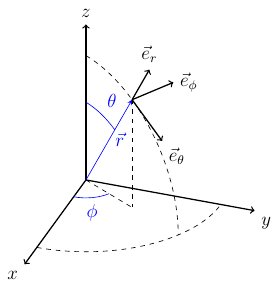
\includegraphics[width=\textwidth]{sketches/spherical_coord2.jpg} 
  \caption*{(b)}
  \end{minipage}
  \caption{(a) Sketch of the liquid outer core. It is bounded by the two spheres of radii R$_i$ and R$_o$. The rotation axis is the cartesian z-axis. (b) This work uses spherical coordinates with unit vectors $ \bm e_r$, $\bm e_\Phi$ and $\bm e_\vartheta$}
\end{figure}

\subsection{Equation of continuity}
Per definition, the mass $ \mathcal{M} $ of a material volume $ \mathcal{V}(t) $ with a density $\rho$, moving with a velocity $ \bm u(\bm r,t) $ in a fluid is conserved: 
\begin{equation}
\frac{d \mathcal{M}(\mathcal{V})}{dt} = \frac{d}{dt} \int_{\mathcal{V}(t)} \rho(\bm r,t) d^3r  = 0
\end{equation}
Using Reynold's Transport Theorem (Appendix ???) and then applying Gauss's Theorem, this yields
\begin{equation}
  \int_{\mathcal{V}(t)} \frac{\partial \rho}{\partial t} d^3r + \int_{\partial \mathcal{V}(t)} \rho \bm u \cdot \bm {ds} = \int_{\mathcal{V}(t)} \left[ \frac{\partial \rho}{\partial t} + \bm \nabla \cdot (\rho \bm u) \right] d^3r = 0.
\end{equation}
Since this has to hold for all possible material volumes $\mathcal V$, one gets
\begin{equation}
 \frac{\partial \rho}{\partial t} + \bm \nabla \cdot (\rho \bm u) = 0,
\end{equation}
the general form of the equation of continuity. The introduction of the \textit{material derivative} $\frac{D }{Dt} = \frac{\partial }{\partial t} + \bm u \cdot \bm \nabla$ suggests another useful formulation:
\begin{equation}
 \frac{\partial \rho}{\partial t} + \rho \bm \nabla \cdot \bm u + \bm u \cdot \bm \nabla \rho =   \frac{D \rho}{D t} + \rho \bm \nabla \cdot \bm u = 0.
\end{equation}


\subsection{Equation of momentum}
In a non-rotating frame of reference, the change of momentum of a material volume $\mathcal{V}$ can be written as 
\begin{align*}
 \frac{d}{dt} \int_{\mathcal{V}(t)} (\rho u_j) d^3r &= \int_{\mathcal{V}(t)} \left[ \frac{\partial (\rho u_j)}{\partial t} + \frac{\partial}{\partial x_i} (\rho u_j)u_i \right]d^3r \\
    &=   \int_{\mathcal{V}(t)} \left[ \rho \frac{\partial u_j}{\partial t} + u_j \frac{\partial \rho}{\partial t}  +\rho u_j \frac{\partial u_i}{\partial x_i} + u_i \rho \frac{\partial u_j}{\partial x_i} + u_i u_j \frac{\partial \rho}{\partial x_i} \right] d^3r\\
    &= \int_{\mathcal{V}(t)} \left[ u_j\left( \frac{\partial \rho}{\partial t} + \rho \bm \nabla \cdot \bm u + \bm u \cdot \bm \nabla \rho \right) + \rho \left( \frac{\partial u_j}{\partial t} + \bm u \cdot \nabla u_j \right) \right]d^3r \\
    &= \int_{\mathcal{V}(t)}  \rho \frac{D \bm u}{D t} d^3r.
\end{align*}
Change of momentum can happen through either \textit{volume forces} $\bm f$ or \textit{surface forces} $\bm g$:
\begin{equation}
 \int_{\mathcal{V}} \rho \frac{D \bm u}{D t} d^3r = \int_{\mathcal{V}} \bm f d^3r + \oint_{\partial \mathcal{V}} \bm g ds
\end{equation}


\subsection{CMB - heat flux pattern}
We impose a heat flux balance between the inner and the outer core boundary. The total influx at the ICB Q$_i$ equals the total outflux Q$_o$ at the CMB:
\begin{align}
 -\textrm{Q}_i &= \textrm{Q}_o\\
 \Leftrightarrow \int \limits_{\Sigma_\textrm{icb}} \kappa \nabla T\big|_\textrm{\tiny{icb}} \cdot \bm e_r dS &= \int \limits_{\Sigma_\textrm{cmb}} \kappa \nabla T\big|_\textrm{\tiny{cmb}} \cdot \bm e_r dS \\
 \Leftrightarrow \int \limits_{\Sigma_\textrm{icb}} \frac{\partial T}{\partial r} \bigg|_\textrm{\tiny{icb}} dS &= \int \limits_{\Sigma_\textrm{cmb}} \frac{\partial T}{\partial r} \bigg|_\textrm{\tiny{cmb}} dS 
\end{align}
For the spectral decomposition it is important to know, that only the 0th order spherical harmonic $\mathcal{Y}_0^0$ yields values $\neq$ 0 when integrated over a closed surface $\Sigma$:
\begin{align}
 \int \limits_{\Sigma} \frac{\partial T}{\partial r} dS = \int \limits_{\Sigma} \left(\frac{\partial T}{\partial r}\right)_0^0 \mathcal{Y}_0^0 dS
\end{align}
with $\left(\frac{\partial T}{\partial r}\right)_0^0$ being the spectral coefficient of degree and order 0.

\begin{align}
 \int \limits_{\Sigma_\textrm{icb}} \left(\frac{\partial T}{\partial r}\right)_0^0\bigg|_\textrm{icb} \mathcal{Y}_0^0 dS &=  \int \limits_{\Sigma_\textrm{cmb}} \left(\frac{\partial T}{\partial r}\right)_0^0\bigg|_\textrm{cmb} \mathcal{Y}_0^0 dS\\
 \Leftrightarrow \left(\frac{\partial T}{\partial r}\right)_0^0\bigg|_\textrm{icb}  r_i^2 &= \left(\frac{\partial T}{\partial r}\right)_0^0\bigg|_\textrm{cmb} r_o^2
\end{align}
This allows to formulate a simple relation between the mean radial temperature gradient at the inner and outer boundary.
\begin{equation}
  \Leftrightarrow \left(\frac{\partial T}{\partial r}\right)_0^0\bigg|_\textrm{icb} = \left(\frac{\partial T}{\partial r}\right)_0^0\bigg|_\textrm{cmb} \frac{r_o^2}{r_i^2} = - \beta \frac{r_o^2}{r_i^2} = - \beta \frac{1}{a^2}
\end{equation}
with $\beta := - \left(\frac{\partial T}{\partial r}\right)_0^0\bigg|_{\textrm{cmb}}$ as prescribed temperature gradient at the CMB.\\
This relation allows us to formulate Neumann boundary conditions for the stationary temperature equation that has the form of a Laplace equation,
\begin{equation}
 \nabla ^2 T = 0 \label{eq:laplace}
\end{equation}
since we have no internal sources.\\
\begin{equation}
 \textrm{ICB:} \quad  \frac{\partial T}{\partial r}\bigg|_{\textrm{icb}} = - \beta \frac{1}{a^2} \mathcal{Y}_0^0 \label{eq:BCicb}
\end{equation}
\begin{equation}
  \textrm{CMB:} \quad \frac{\partial T}{\partial r}\bigg|_{\textrm{cmb}} = - \beta \mathcal{Y}_0^0 + Amp_l^m \mathcal{Y}_l^m \label{eq:BCcmb}
\end{equation}
where $Amp_l^m$ is the amplitude of the heat flux heterogeneity.\\
The general solution of \eqref{eq:laplace} in spherical coordinates reads
\begin{equation}
 T = \sum \limits_{l,m} \left[ a_l^m r^l + b_l^m r^{-l-1} \right] \mathcal{Y}_l^m(\vartheta,\varphi) \label{eq:cond}
\end{equation}
and its radial derivative 
\begin{equation}
\frac{\partial T}{\partial r} = \sum \limits_{l,m} \left[l a_l^m r^{l-1} - (l+1) b_l^m r^{-l-2}\right]  \mathcal{Y}_l^m(\vartheta,\varphi). \label{eq:gradcond}
\end{equation}
From \eqref{eq:BCicb} and \eqref{eq:gradcond} follows immediately for $l=m=0$
\begin{equation}
 - b_0^0 r_i^{-2} = -\beta \frac{1}{a^2} \quad \Rightarrow \quad b_0^0 = \beta r_o^2
\end{equation}
and the algebraic equation 
\begin{equation}
 la_l^m r_i^{l-1} - (l+1) b_l^m r_i^{-l-2} = 0 \label{eq:algebraicICB}
\end{equation}
for all $l>0$ and $m>0$.\\
\eqref{eq:BCcmb} and \eqref{eq:cond} together give another equation for the determination of $a_l^m$ and $b_l^m$:
\begin{equation}
 l a_l^m r_o^{l-1} - (l+1)b_l^m r_o^{-l-2} = Amp_l^m. \label{eq:algebraicCMB}
\end{equation}
Since only a heat flux pattern with $l=m=2$ will be used here, \eqref{eq:algebraicICB} and \eqref{eq:algebraicCMB} simplify to
\begin{equation}
 \left( \begin{matrix} 2r_o & -3r_o^{-4}\\ 2r_i & -3r_i^{-4}\end{matrix} \right) \left(\begin{matrix} a_2^2\\b_2^2 \end{matrix}\right) = \left( \begin{matrix} Amp_2^2 \\ 0 \end{matrix} \right).                                                                                                                                                
\end{equation}
In a nondimensional form, the solution \eqref{eq:laplace} is
\begin{equation}
 \hat{T} = \frac{T}{d\beta} = \left( \frac{a_0^0}{d\beta} + \frac{1}{(a-1)^2\hat{r}} \right) \mathcal{Y}_0^0 + \frac{Amp_2^2}{\beta}\cdot \frac{2a^5\hat{r}^3 - 3(a-1)^5\hat{r}^2}{6(a-1)^4(1-a^5)} \mathcal{Y}_2^2
\end{equation}
with $a_0^0$ being an arbitrary integration constant that is chosen to be 0 in the following.


\newpage
% \bibliography{literatur}
% \bibliographystyle{apalike}
%\bibitem[1]{literatur} Experimentellen

%\end{thebibliography}
\end{document}